% !TeX root = ../main.tex

% Edit this title for each week's entry.
\section{Week 7 - Depreciation}

\topic{Introduction and Overview}

\begin{example}[Motivating Example]
    A machine is purchased for \$100,000, loses \$15,000 in value every year,
    and is sold after 5 years for \$25,000. Identify the cost concepts that
    appear in this example.
    \begin{itemize}
        \item \db{\$100,000: the \dbb{first cost} (a cash-flow at $t = 0$)}
        \item \db{\$15,000/year: the \dbb{depreciation} (loss in value each year, \emph{not} a cash-flow)}
        \item \db{\$25,000: the \dbb{salvage value} (a cash-flow at $t = 5$). It matches the value left on the books: $100{,}000 - 5(15{,}000) = 25{,}000$}
    \end{itemize}
\end{example}

\begin{definition}[Depreciation]
    From the Oxford English Dictionary:
    \begin{enumerate}
        \item ``\dbb{Diminish in value} over a period of time''
        \item ``Reduce the \dbb{recorded value} of an asset over a predetermined period''
    \end{enumerate}
\end{definition}

\begin{example}[Reflection: Losing Value]
    An asset starts to lose value as soon as it is purchased. Why?
    \\\db{It starts wearing out and ageing, and newer, better models keep appearing. A used asset is also worth less to a buyer than a new one.}
\end{example}

\heading{Reasons for Depreciation}
\b{Assets deteriorate}:
\begin{itemize}
    \item \rb{Use-related physical loss}: as something is used, its parts wear out (``wear and tear'')
    \item \rb{Time-related physical loss}: even if not used, things deteriorate with time as nature or other effects take their toll
\end{itemize}
\b{Assets become obsolete}:
\begin{itemize}
    \item \rb{Functionality-related loss}: loss that occurs \dbb{without any physical changes} (e.g.\ a newer, faster model makes the old one less useful)
\end{itemize}

\begin{definition}[Depreciation in Accounting]
    A procedure where the cost of an asset \dbb{less its estimated salvage
    value} is distributed over the asset's estimated useful life in a
    systematic and rational manner.
\end{definition}

\begin{center}
    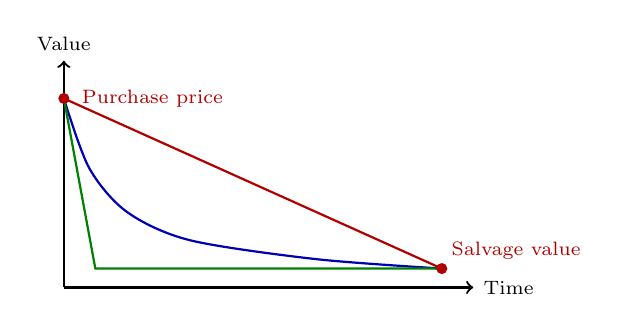
\begin{tikzpicture}[scale=0.8]
        \draw[->,thick] (0,0) -- (6.5,0) node[right] {\scriptsize Time};
        \draw[->,thick] (0,0) -- (0,3.6) node[above] {\scriptsize Value};
        \draw[red!70!black,thick] (0,3) -- (6,0.3);
        \draw[blue!70!black,thick] plot[smooth] coordinates {(0,3) (0.4,1.9) (1,1.2) (2,0.75) (4,0.45) (6,0.3)};
        \draw[green!50!black,thick] (0,3) -- (0.5,0.3) -- (6,0.3);
        \fill[red!70!black] (0,3) circle (2.5pt) node[right=3pt] {\scriptsize Purchase price};
        \fill[red!70!black] (6,0.3) circle (2.5pt) node[above right] {\scriptsize Salvage value};
    \end{tikzpicture}
    \\[2pt] \textit{\small Different methods spread the same total loss $B - S$ differently over time}
\end{center}

\begin{example}[Reflection: Cash-flow Diagram]
    How do we show this situation (purchase price falling to a salvage
    value) on a cash-flow diagram?
    \\\db{Only the money that actually changes hands appears: the purchase price at $t = 0$ and the salvage value at $t = N$. The gradual loss of value in between is \dbb{not} drawn.}
    \begin{center}
        \begin{tikzpicture}[scale=0.8]
            \draw[->] (0,0) -- (6.5,0) node[right] {\scriptsize $t$};
            \draw[->,thick,red!70!black] (0,0) -- (0,-1.5) node[below] {\scriptsize Purchase price};
            \draw[->,thick,green!50!black] (6,0) -- (6,0.6) node[above] {\scriptsize Salvage value};
            \node[below] at (6,-0.05) {\scriptsize $N$};
        \end{tikzpicture}
    \end{center}
\end{example}

\begin{remark}[Depreciation Is Not a Cash-flow]
    \begin{itemize}
        \item Depreciation is an accounting ``fiction'' from an engineering economics point of view
        \item In engineering economics, the purchase is treated as a cash-flow at time 0 and then as a cost of capital over its life (as we saw before)
        \item Depreciation does \textbf{not} involve any cash-flows, so it does \textbf{not} enter directly into our calculations
    \end{itemize}
\end{remark}

\heading{Why Does Depreciation Matter?}
\begin{itemize}
    \item Internal company book-keeping and financial planning
    \item Financial reporting: useful for investors and company valuation
    \item Assets can be used as collateral for loans
    \item \b{Tax implications}
\end{itemize}

\heading{What Do We Mean by ``Value''?}
\begin{itemize}
    \item \rb{Cost basis}: the value against which depreciation is measured. Usually based on first costs
    \item \rb{Market value}: the actual value of an asset if sold in a free market. Usually can't be observed directly unless the item is actually sold
    \item \rb{Book value}: the value calculated for accounting purposes according to an agreed-upon model (\dbb{the focus of this section})
\end{itemize}

\heading{Key Symbols}
\begin{itemize}
    \item $B$: basis
    \item $BV_t$: book value at time $t$
    \item $N$: depreciable life of the asset (NB: not necessarily equal to the asset's \emph{useful} life)
    \item $S$: salvage value
    \item $D_t$: the loss of value assigned to accounting period $t$
\end{itemize}
The book value in year 0 is usually the cost basis, and it changes each year
by the amount of depreciation:
\[\boxed{BV_0 = B, \qquad BV_t = BV_{t-1} - D_t = B - \sum_{j=1}^{t} D_j}\]

\heading{Depreciation Methods}
\begin{itemize}
    \item There are many methods: \b{straight-line}, \b{declining-balance}, double-declining-balance, sum-of-the-years'-digits, units-of-production
    \item They are mostly \dbb{arbitrary conventions}, but are important for accounting and tax purposes. Firms can choose which method to report
    \item The government usually specifies allowed/required methods of depreciation for tax purposes
\end{itemize}

\heading{Costs to Include in Depreciation}
Include all costs necessary to bring the asset to its \dbb{intended use and
condition}:
\begin{itemize}
    \item Purchase price; duties and taxes; transportation and handling
    \item Installation and assembly; testing and calibration
    \item Professional fees; initial spare parts and accessories
\end{itemize}

\heading{Summary}
\begin{enumerate}
    \item Depreciation is the loss in value of an asset over time, \b{or} an accounting method to reduce the recorded value of an asset over a predetermined period
    \item Reasons: use-related, time-related, or functionality-related loss
    \item Value concepts: cost basis, market value, and book value
    \item Depreciation is \b{not} a cash-flow!
\end{enumerate}

\topic{Straight-Line and Declining Balance}

\begin{definition}[Straight-Line (SL) Depreciation]
    The simplest and best-known method. Assumes the annual loss in value is
    \dbb{constant} over the asset's life:
    \[\boxed{\begin{gathered}
        D_t = \frac{B - S}{N}, \qquad BV_t = B - \frac{t(B - S)}{N}\\[4pt]
        \begin{array}{@{}l@{}}
            B: \text{basis } (= BV_0)\\
            S: \text{salvage value}\\
            N: \text{depreciable life}\\
            D_t: \text{depreciation in year } t
        \end{array}
    \end{gathered}}\]
\end{definition}

\begin{example}[Straight Line]
    The Gigabit software company has purchased a server for \$250,000. It
    is expected to last 6 years, with a salvage value of \$10,000. Use
    straight-line depreciation to calculate:
    \begin{enumerate}[label = \roman*.]
        \item The depreciation amount for year 1
        \[D_1 = \frac{250{,}000 - 10{,}000}{6} = \db{\$40{,}000}\]
        \item The depreciation amount for year 6
        \\\db{SL is constant every year: $D_6 = \$40{,}000$.}
        \item The book value at the end of year 4
        \[BV_4 = 250{,}000 - 4(40{,}000) = \db{\$90{,}000}\]
        \item The accumulated depreciation at the end of year 4
        \[\sum_{t=1}^{4} D_t = 4(40{,}000) = B - BV_4 = \db{\$160{,}000}\]
    \end{enumerate}
\end{example}

\begin{definition}[Declining Balance (DB) Depreciation]
    The most common method required by the Canadian government for tax
    purposes. The loss in value is modelled as a \dbb{constant proportion}
    $d$ of the asset's book value at the start of each year:
    \[\boxed{\begin{gathered}
        D_t = BV_{t-1}\,d, \qquad BV_t = B(1 - d)^t\\[4pt]
        \begin{array}{@{}l@{}}
            d: \text{depreciation rate}\\
            B: \text{basis}\\
            BV_{t-1}: \text{book value at the end of year } t-1
        \end{array}
    \end{gathered}}\]
\end{definition}

\begin{example}[Declining Balance]
    An asset is purchased for \$900, with a declining-balance rate of 40\%
    ($d = 0.4$) and $N = 5$.
    \begin{center}
    \begin{tabular}{cccc}
        \toprule
        $t$ & $D_t$ & $\sum D_t$ & $BV_t$ \\
        \midrule
        1 & $0.4(900) = 360$ & 360 & 540 \\
        2 & $0.4(540) = 216$ & 576 & 324 \\
        3 & $0.4(324) = 129.60$ & 705.60 & 194.40 \\
        4 & $0.4(194.40) = 77.76$ & 783.36 & 116.64 \\
        5 & $0.4(116.64) = 46.66$ & 830.02 & 69.98 \\
        \bottomrule
    \end{tabular}
    \end{center}
    \db{Check: $BV_5 = 900(0.6)^5 = 69.98$.}
\end{example}

\begin{example}[Declining Balance: Computers]
    A company purchases small computers for \$7,000 each. They are expected
    to last 5 years. Use a DB rate of 40\% to determine:
    \begin{enumerate}[label = \alph*)]
        \item The depreciation charge during year 1
        \[D_1 = 0.4(7000) = \db{\$2800}\]
        \item The depreciation charge during year 2
        \[D_2 = 0.4\,BV_1 = 0.4(7000 - 2800) = \db{\$1680}\]
        \item The book value at the end of year 3
        \[BV_3 = 7000(1 - 0.4)^3 = \db{\$1512}\]
    \end{enumerate}
\end{example}

\begin{example}[Reflection: What Is Wrong?]
    Company X purchased an asset for \$10,000 with a useful life of 5 years.
    The depreciation rate is 20\% and the salvage value is \$1000 by the end
    of 5 years. What is wrong with this problem statement?
    \\\db{It is \dbb{over-specified}: $B$, $N$, $d$ and $S$ cannot all be chosen freely. With $d = 20\%$:}
    \[BV_5 = 10{,}000(0.8)^5 = \$3276.80 \neq \$1000\]
    \db{To fix it, drop one of the conditions. If $S = \$1000$ at $N = 5$ is right, the rate must be}
    \[d = 1 - \sqrt[5]{1000/10{,}000} = 36.9\%\]
    \db{or, keeping $d = 20\%$, the book value after 5 years must be \$3276.80.}
\end{example}

\heading{Declining Balance Rate Selection}
If the salvage value is known, choose $d$ so that the book value reaches $S$
after $N$ years:
\[B(1 - d)^N = S \quad\Longrightarrow\quad \boxed{d = 1 - \sqrt[N]{\frac{S}{B}}}\]

\begin{example}[Choosing a DB Rate]
    An asset is purchased for \$8,000, with a depreciable life of 7 years and
    a salvage value of \$900. What is an appropriate DB rate?
    \[d = 1 - \sqrt[7]{\frac{900}{8000}} = 1 - 0.7319 = \db{26.8\%}\]
\end{example}

\begin{example}[Reflection: Reaching Zero]
    Under declining balance depreciation, when does the asset's value drop
    to 0?
    \\\db{\dbb{Never} (for $d < 1$): $BV_t = B(1 - d)^t > 0$ for every $t$. The book value only approaches 0 as $t \to \infty$. So DB can't be used with $S = 0$ in the formula for $d$.}
\end{example}

\begin{center}
    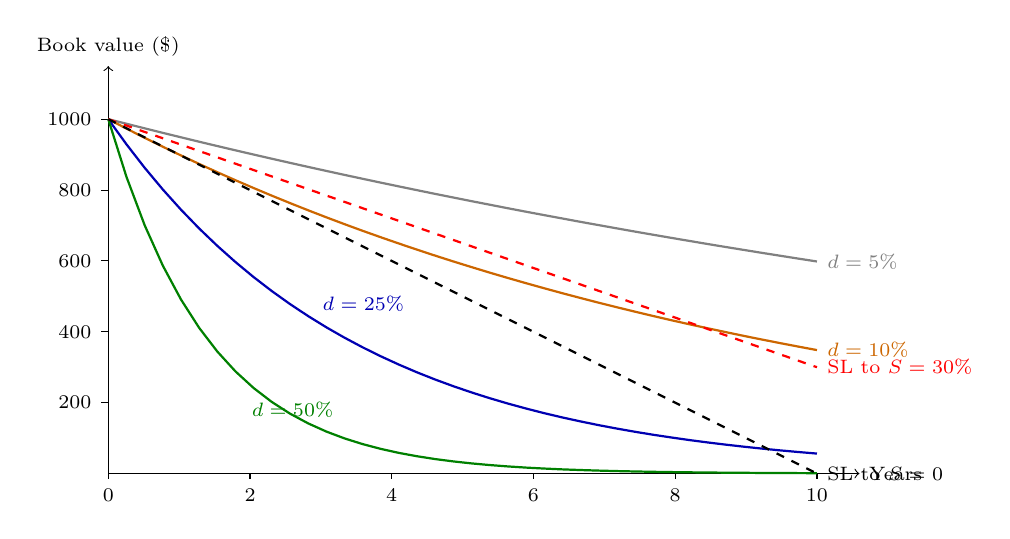
\begin{tikzpicture}[xscale=0.9, yscale=0.9]
        % y in units of $200 (1 unit = $200)
        \draw[->] (0,0) -- (10.6,0) node[right] {\scriptsize Years};
        \draw[->] (0,0) -- (0,5.75) node[above] {\scriptsize Book value (\$)};
        \foreach \x in {0,2,...,10}{\draw (\x,0) -- (\x,-0.08) node[below] {\scriptsize \x};}
        \foreach \v in {1,...,5}{\draw (0,\v) -- (-0.1,\v) node[left] {\scriptsize \pgfmathparse{int(\v*200)}\pgfmathresult};}
        \draw[thick,gray,domain=0:10,samples=40] plot (\x,{5*0.95^\x}) node[right] {\scriptsize $d = 5\%$};
        \draw[thick,orange!80!black,domain=0:10,samples=40] plot (\x,{5*0.9^\x}) node[right] {\scriptsize $d = 10\%$};
        \draw[thick,blue!70!black,domain=0:10,samples=40] plot (\x,{5*0.75^\x});
        \node[blue!70!black] at (3.6,2.4) {\scriptsize $d = 25\%$};
        \draw[thick,green!50!black,domain=0:10,samples=40] plot (\x,{5*0.5^\x});
        \node[green!50!black] at (2.6,0.9) {\scriptsize $d = 50\%$};
        \draw[thick,dashed,red] (0,5) -- (10,1.5) node[right] {\scriptsize SL to $S = 30\%$};
        \draw[thick,dashed] (0,5) -- (10,0) node[right] {\scriptsize SL to $S = 0$};
    \end{tikzpicture}
    \\[2pt] \textit{\small Book value against time ($B = \$1000$, $N = 10$)}
\end{center}

\begin{definition}[Double Declining Balance (DDB)]
    A version of DB, sometimes called the \rb{200\% method}. It can be used
    when $N$ is known:
    \[\boxed{d = \frac{2}{N}}\]
    E.g.\ if $N = 10$, then $d = 2/10 = 20\%$ of the book value is written
    off each year (\dbb{double} the SL rate of $1/N$).
\end{definition}

\heading{Summary}
\begin{enumerate}
    \item \b{Straight-line}: constant annual loss, $D_t = (B - S)/N$ and $BV_t = B - t(B - S)/N$
    \item \b{Declining balance}: $D_t = BV_{t-1}\,d$ and $BV_t = B(1 - d)^t$. If $S$ is known, $d = 1 - \sqrt[N]{S/B}$. DDB uses $d = 2/N$
\end{enumerate}

\topic{Sum-of-Years'-Digits and Units of Production}

Both methods divide the lifetime depreciation $B - S$ into parts:
\begin{enumerate}
    \item Divide into arbitrary parts: \rb{sum-of-years'-digits}
    \item Divide into parts based on production: \rb{units of production}
\end{enumerate}

\begin{definition}[Sum-of-Years'-Digits (SOYD)]
    The SOYD is $1 + 2 + \dots + N = N(N+1)/2$ (e.g.\ for $N = 5$, SOYD
    $= 15$). Year $t$ gets the fraction $(N - t + 1)/\text{SOYD}$ of the
    total loss:
    \[\boxed{\begin{gathered}
        D_t = \frac{N - t + 1}{\text{SOYD}}(B - S)\\[4pt]
        \begin{array}{@{}l@{}}
            \text{SOYD}: 1 + 2 + \dots + N\\
            N: \text{depreciable life}\\
            B - S: \text{total loss in value}
        \end{array}
    \end{gathered}}\]
    Faster than straight line in the \dbb{early} years, and slower in the
    \dbb{later} years.
\end{definition}

\begin{example}[SOYD Depreciation]
    An asset is purchased for \$900 and depreciates to $S = \$70$ over 5
    years, so $B - S = \$830$ and SOYD $= 15$.
    \begin{center}
    \begin{tabular}{ccccc}
        \toprule
        $t$ & Rate & $D_t$ & $\sum D_t$ & $BV_t$ \\
        \midrule
        1 & 5/15 & $\frac{5}{15}(830) = 277$ & 277 & 623 \\
        2 & 4/15 & $\frac{4}{15}(830) = 221$ & 498 & 402 \\
        3 & 3/15 & $\frac{3}{15}(830) = 166$ & 664 & 236 \\
        4 & 2/15 & $\frac{2}{15}(830) = 111$ & 775 & 125 \\
        5 & 1/15 & $\frac{1}{15}(830) = 55$ & 830 & 70 \\
        \bottomrule
    \end{tabular}
    \end{center}
    \db{The book value lands exactly on $S$ after $N$ years.}
\end{example}

\begin{definition}[Units of Production]
    Assumes depreciation is a function of \dbb{equipment use} rather than
    time:
    \[\boxed{D_t = \frac{\text{production in year } t}{\text{lifetime production}}(B - S)}\]
\end{definition}

\begin{example}[Units of Production Depreciation]
    A machine is purchased for \$10,000 and will last for 50,000 units
    ($S = 0$).
    \\\db{The machine depreciates by $10{,}000/50{,}000 = \$0.20$ per unit.}
    \begin{center}
    \begin{tabular}{ccccc}
        \toprule
        $t$ & Units made & $D_t$ & $\sum D_t$ & $BV_t$ \\
        \midrule
        1 & 15,000 & \$3000 & \$3000 & \$7000 \\
        2 & 12,500 & \$2500 & \$5500 & \$4500 \\
        3 & 10,000 & \$2000 & \$7500 & \$2500 \\
        4 & 7,500 & \$1500 & \$9000 & \$1000 \\
        5 & 5,000 & \$1000 & \$10,000 & \$0 \\
        \bottomrule
    \end{tabular}
    \end{center}
\end{example}

\heading{Summary}
\begin{enumerate}
    \item \b{SOYD}: $D_t = \frac{N - t + 1}{\text{SOYD}}(B - S)$
    \item \b{Units of production}: $D_t = \frac{\text{production in year } t}{\text{lifetime production}}(B - S)$
\end{enumerate}

\topic{Adjusting for Asset End of Life}

\heading{When Market Value Differs from Book Value}
When the asset is sold, its market value (= the actual salvage value) rarely
equals its book value. The difference is booked as a one-time adjustment:
\begin{center}
    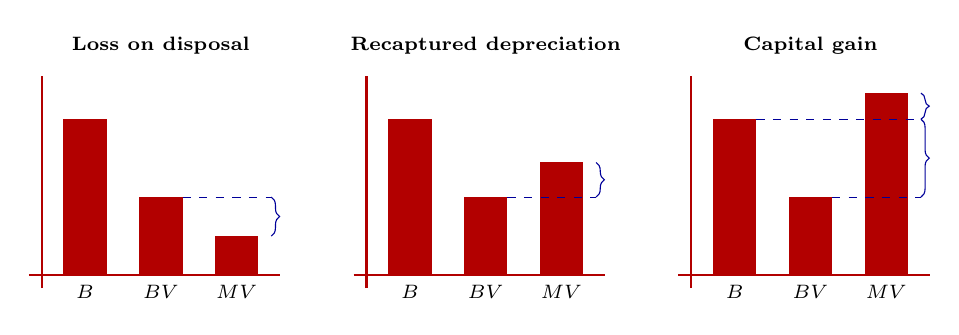
\begin{tikzpicture}[scale=0.55, every node/.style={font=\scriptsize}]
        \foreach \dx/\mv/\title in {0/0.9/Loss on disposal, 7.5/2.6/Recaptured depreciation, 15/4.2/Capital gain}{
            \begin{scope}[xshift=\dx cm]
                \draw[thick,red!70!black] (-0.3,0) -- (5.5,0);
                \draw[thick,red!70!black] (0,-0.3) -- (0,4.6);
                \fill[red!70!black] (0.5,0) rectangle (1.5,3.6);
                \fill[red!70!black] (2.25,0) rectangle (3.25,1.8);
                \fill[red!70!black] (4,0) rectangle (5,\mv);
                \node[below] at (1,0) {$B$};
                \node[below] at (2.75,0) {$BV$};
                \node[below] at (4.5,0) {$MV$};
                \node at (2.75,5.3) {\textbf{\title}};
            \end{scope}
        }
        \draw[dashed,blue!60!black] (3.25,1.8) -- (5.3,1.8);
        \draw[decorate,decoration={brace,amplitude=3pt},blue!60!black] (5.3,1.8) -- (5.3,0.9);
        \draw[dashed,blue!60!black] (10.75,1.8) -- (12.8,1.8);
        \draw[decorate,decoration={brace,amplitude=3pt},blue!60!black] (12.8,2.6) -- (12.8,1.8);
        \draw[dashed,blue!60!black] (18.25,1.8) -- (20.3,1.8);
        \draw[dashed,blue!60!black] (16.5,3.6) -- (20.3,3.6);
        \draw[decorate,decoration={brace,amplitude=3pt},blue!60!black] (20.3,3.6) -- (20.3,1.8);
        \draw[decorate,decoration={brace,amplitude=3pt},blue!60!black] (20.3,4.2) -- (20.3,3.6);
    \end{tikzpicture}
    \\[2pt] \textit{\small $B$ = cost basis, $BV$ = book value, $MV$ = market value = salvage value}
\end{center}
\begin{itemize}
    \item \rb{Loss on disposal} ($MV < BV$): a one-time \dbb{additional} depreciation when sold
    \item \rb{Recaptured depreciation} ($MV > BV$): a one-time \dbb{negative} depreciation. The asset was depreciated too fast on the books
    \item \rb{Capital gain} ($MV > B$): the part of the sale price \dbb{above the cost basis}. The part between $BV$ and $B$ is still recaptured depreciation
\end{itemize}

\heading{Reconciling Book Value with the True Salvage Value}
\begin{itemize}
    \item Market value differs from book value at sale $\to$ \b{adjust for the difference} (disposal loss or recaptured depreciation)
    \item Service life differs $\to$ \b{re-evaluate the useful life}: from that point on, depreciate the current book value over the new remaining life
\end{itemize}
\begin{center}
    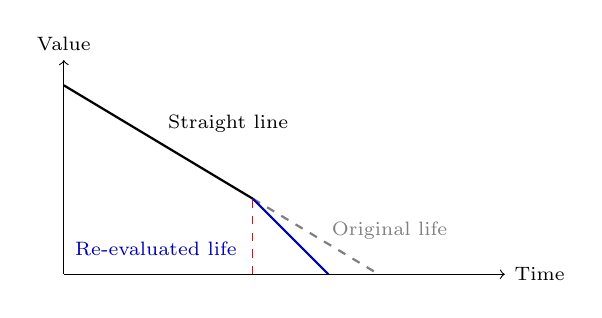
\begin{tikzpicture}[scale=0.8]
        \draw[->] (0,0) -- (7,0) node[right] {\scriptsize Time};
        \draw[->] (0,0) -- (0,3.4) node[above] {\scriptsize Value};
        \draw[thick] (0,3) -- (3,1.2);
        \draw[thick,dashed,gray] (3,1.2) -- (5,0);
        \draw[thick,blue!70!black] (3,1.2) -- (4.2,0);
        \draw[dashed,red] (3,0) -- (3,1.2);
        \node[above right] at (1.5,2.1) {\scriptsize Straight line};
        \node[left,blue!70!black] at (2.9,0.4) {\scriptsize Re-evaluated life};
        \node[right,gray] at (4.1,0.7) {\scriptsize Original life};
    \end{tikzpicture}
\end{center}

\begin{example}[Loss at Disposal]
    An asset is purchased for \$900, with a DB rate of 40\%, $N = 5$ and
    \b{no salvage value}.
    \begin{center}
    \begin{tabular}{cccc}
        \toprule
        $t$ & $D_t$ & $\sum D_t$ & $BV_t$ \\
        \midrule
        1 & 360 & 360 & 540 \\
        2 & 216 & 576 & 324 \\
        3 & 129.60 & 705.60 & 194.40 \\
        4 & 77.76 & 783.36 & 116.64 \\
        5 & \db{116.64} & \db{900} & \db{0} \\
        \bottomrule
    \end{tabular}
    \end{center}
    \db{DB never reaches 0 on its own, so in year 5 the whole remaining book value \$116.64 is written off as a \dbb{loss on disposal}. Total depreciation is the full \$900.}
\end{example}

\begin{example}[Recaptured Depreciation]
    Same asset (\$900, $d = 0.4$, $N = 5$), but it sells for \b{\$300} at
    the end of year 5.
    \begin{center}
    \begin{tabular}{cccc}
        \toprule
        $t$ & $D_t$ & $\sum D_t$ & $BV_t$ \\
        \midrule
        1--4 & (as above) & 783.36 & 116.64 \\
        5 & \db{$-183.36$} & \db{600} & \db{300} \\
        \bottomrule
    \end{tabular}
    \end{center}
    \db{The asset is worth more than its book value, so the books are moved \emph{up} to \$300. Year 5 has a negative depreciation of $116.64 - 300 = -\$183.36$ (\dbb{recaptured depreciation}). Total depreciation is $900 - 300 = \$600$.}
\end{example}

\begin{example}[Re-evaluated Service Life]
    An asset is purchased for \$1500 and is expected to last 15 years with no
    salvage value. After 6 years, maintenance realizes the asset is
    degrading and will only last \b{another 4 years}. The company uses
    straight-line depreciation. What is the book value at the end of year 8?
    \\\db{Years 1--6 at the original rate:}
    \[D = \frac{1500 - 0}{15} = \$100/\text{yr}, \qquad BV_6 = 1500 - 6(100) = \$900\]
    \db{From year 7, depreciate the remaining \$900 over the new remaining life of 4 years:}
    \[D' = \frac{900 - 0}{4} = \$225/\text{yr}, \qquad BV_8 = 900 - 2(225) = \db{\$450}\]
\end{example}

\heading{Summary}
\begin{enumerate}
    \item Market value differs at sale $\to$ reconcile the book value with the true salvage value:
    \begin{itemize}
        \item Salvage $<$ book value: \b{loss on disposal}
        \item Salvage $>$ book value: \b{recaptured depreciation}
        \item Salvage $>$ first cost: \b{capital gain}
    \end{itemize}
    \item Service life differs $\to$ re-evaluate the useful life
\end{enumerate}
